%%
%  ******************************************************************************
%  * #file    Szablon_raportu_EN_Latex.tex
%  * #author  Adrian Wójcik   adrian.wojcik(at)put.poznan.pl
%  *          
%  * #commit  Patryk Kościk   koscikpatryk(at)gmail.com
%  *          Modified the template for Projekt przejsciowy purposes          
%  *          
%  *
%  * #commit  Patryk Kościk   koscikpatryk(at)gmail.com
%  *          Zupełnie przewrócono na łeb formatke po taktycznym wyjasnieniu          
%  *          
%  * #version 1.1
%  * #date    09-Mar-2022
%  * #brief   PROJPRZEJ
%  *
%  ******************************************************************************
%%  
\documentclass[11pt, a4paper]{article}

\usepackage{SM_template}

% Wypełnijcie te dyrektywy zgodnie z waszym tematem
%
% \lab      -> NAZWA CZUJNIKA,          np.: 'DHT22'
% \comment  -> Króciutki opis co to,    np.: 'Cyfrowy czujnik temperatury'
% \author   -> Autor dokumentu          np.: Patryk Kościk
%
% Pamiętajcie o zmianie ścieżki w \addbibresourcue (!)

\lab{Moduł DS18B20}
\comment{Cyfrowy czujnik temperatury}
\author{Anna Nasierowska}
\addbibresource{bib/DS18B20.bib}

%
% Początek dokumentu
%
\begin{document}

%
% Strona tytułowa
%
\mainpage{fig/DS18B20/tytul.png}
\newpage

\section*{Opis elementu}
Omawiany czujnik to cyfrowy termometr umieszczony w obudowie typowej dla tranzystorów. Ma on 3 nóżki, z czego tylko jedna z nich to pin sygnałowy, dwie pozostałe są podłączane do napięcia i masy. Ze względu na to, że jest to czujnik cyfrowy, na jego wyjście podawany jest sygnał binarny, którego wartość temperatury odczytuje się za pomocą komunikacji protokołem One Wire. Składa się on z sensora temperatury, pamięci ROM, rejestru oraz 2 wyzwalaczy alarmów dla niskiej i wysokiej temperatury. 

%%%%%%%%%%%%%%%%%%%%%%%%%  TWO IMAGES SIDE BY SIDE  %%%%%%%%%%%%%%%%%%%%%%%%%%%%%
\vspace{0.25cm}
\begin{figure}[h]
\centering
%%%%%%%%%%%%%%%%%%%%%%%%%%%%%%%%%%%%%%%%%%%%%%%%%%%%%%%%%%%%%%%%%%%%%%%%%%%%%%%%%
\begin{subfigure}{.5\textwidth}
\centering
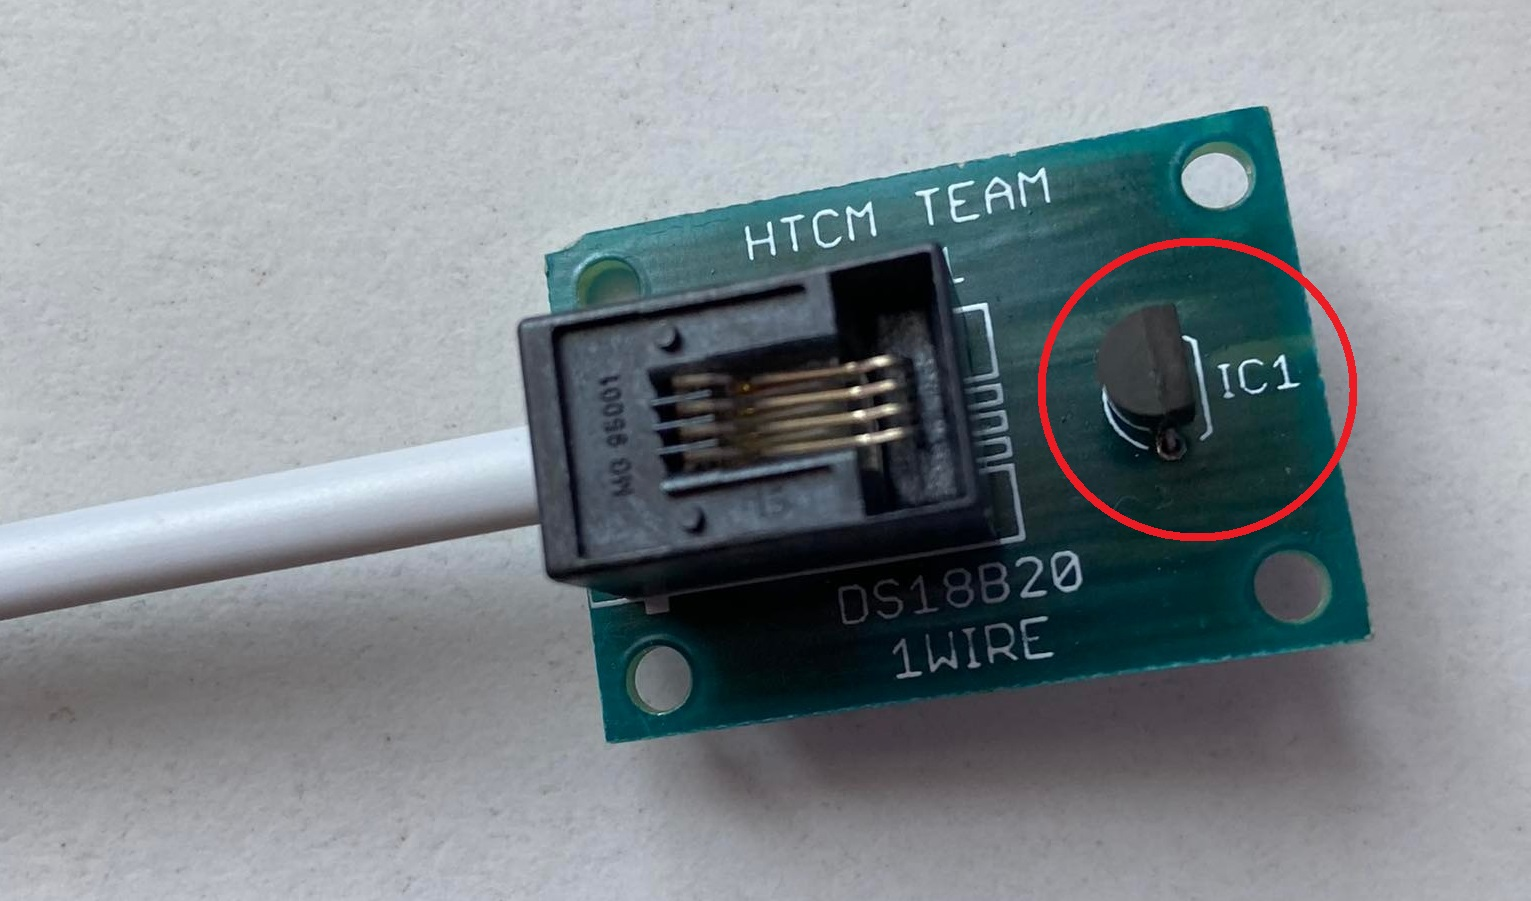
\includegraphics[width=0.8\linewidth]{fig/DS18B20/zdj_modułu/zdj.jpg}
\caption{Zdjęcie modułu z zaznaczonym czujnikiem}
\label{fig:_zdjecie_elementu}
\end{subfigure}%
%%%%%%%%%%%%%%%%%%%%%%%%%%%%%%%%%%%%%%%%%%%%%%%%%%%%%%%%%%%%%%%%%%%%%%%%%%%%%%%%%
\begin{subfigure}{.5\textwidth}
\centering
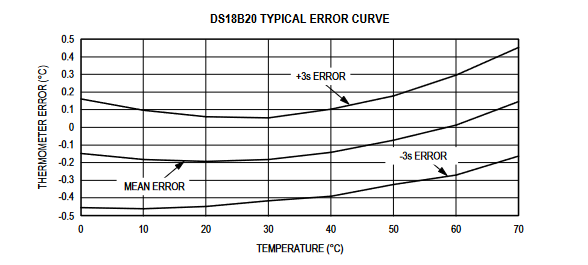
\includegraphics[width=\linewidth]{fig/DS18B20/zasada_dzialania/char.png}
\caption{Charakterystyka błędu pomiarowego czujnika.}
\label{fig:_zasada_dzialania_elementu}
\end{subfigure}
%%%%%%%%%%%%%%%%%%%%%%%%%%%%%%%%%%%%%%%%%%%%%%%%%%%%%%%%%%%%%%%%%%%%%%%%%%%%%%%%%
% \caption{PODPIS}
\label{fig:element}
\end{figure}
\vspace{0.25cm}
%%%%%%%%%%%%%%%%%%%%%%%%%  TWO IMAGES SIDE BY SIDE  %%%%%%%%%%%%%%%%%%%%%%%%%%%%%



% \subsection{Opis modułu} REPLACE SUBSECTION WITH 1CM VSPACE
\vspace{0.75cm}

Moduł omawiany w tym dokumencie to bardzo prosty układ, gdyż składa się on tylko z czujnika i gniazda dla złącza typu RJ. 
Wszystkie 3 nóżki czujnika są połączone ze złączem, które wchodzą do jednego przewodu. 

%%%%%%%%%%%%%%%%%%%%%%%%%  TWO IMAGES SIDE BY SIDE  %%%%%%%%%%%%%%%%%%%%%%%%%%%%%
\begin{figure}[h]
\centering
%%%%%%%%%%%%%%%%%%%%%%%%%%%%%%%%%%%%%%%%%%%%%%%%%%%%%%%%%%%%%%%%%%%%%%%%%%%%%%%%%
\begin{subfigure}{.5\textwidth}
\centering
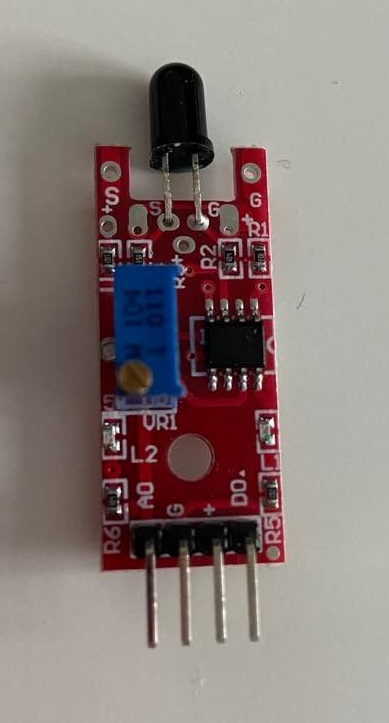
\includegraphics[width=0.9\linewidth]{fig/DS18B20/zdj_modułu/zdj2.jpg}
\caption{Zdjęcie modułu}
\label{fig:_zdjecie_modulu}
\end{subfigure}%
%%%%%%%%%%%%%%%%%%%%%%%%%%%%%%%%%%%%%%%%%%%%%%%%%%%%%%%%%%%%%%%%%%%%%%%%%%%%%%%%%
\begin{subfigure}{.5\textwidth}
\centering
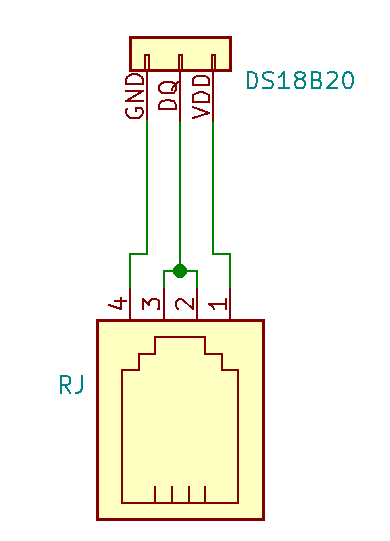
\includegraphics[width=.6\linewidth]{fig/DS18B20/polaczenie_modulu/schem.png}
\caption{Schemat elektryczny modułu}
\label{fig:_schemat_modulu}
\end{subfigure}
%%%%%%%%%%%%%%%%%%%%%%%%%%%%%%%%%%%%%%%%%%%%%%%%%%%%%%%%%%%%%%%%%%%%%%%%%%%%%%%%%
\label{fig:modul}
\end{figure}
\vspace{0.5cm}
%%%%%%%%%%%%%%%%%%%%%%%%%  TWO IMAGES SIDE BY SIDE  %%%%%%%%%%%%%%%%%%%%%%%%%%%%%

Pomiar wykonuje się jak najbardziej przybliżając przedmiot do czujnika. Czujnik zawiera w sobie oscylatory krystaliczne: jeden z niskim, a drugi z wysokim współczynnikiem temperaturowym. Jeden generator impulsów zapewnia stałą pulsację, a drugi - z wysokim współczynnikiem - jest wysoko wrażliwy na zmianę temperatury i zmienia częstotliwość impulsów zależnie od niej. Do oscylatorów podłączone są liczniki zliczające impulsy, których wartości odejmuje się od siebie, a wynik tej operacji przekazywany jest do rejestru temperatury. Do tego dochodzi jeszcze bramka licznikowa, która kontroluje kiedy wykonywać zliczanie. Proces pomiaru temperatury jest nieliniowy, jednak w celu zniwelowania tej nieliniowości w układzie oscylatorów i liczników, zamieszczony jest na wejście do komparatora razem z wyjściem z licznika akumulator rampowy. W ten sposób, pomiar temperatury jest zlinearyzowany i od razu konwertowany na wartość cyfrową. \\
Czujnik ma zastosowanie zarówno w przemyśle, np. w termo wrażliwych systemach automatyki, jak i w produktach konsumenckich takich jak termometry cyfrowe. 



\section{Użycie czujnika}

Moduł podłączono do płytki NUCLEO-F767ZI, do masy, napięcia +5V oraz nóżkę sygnałową do pinu PE2, z rezystorem podciągającym o oporności 4.7k Ohm. Podłączenie na zdjęciu poniżej: 
\begin{figure}[h]
\begin{subfigure}{.5\textwidth}
\centering
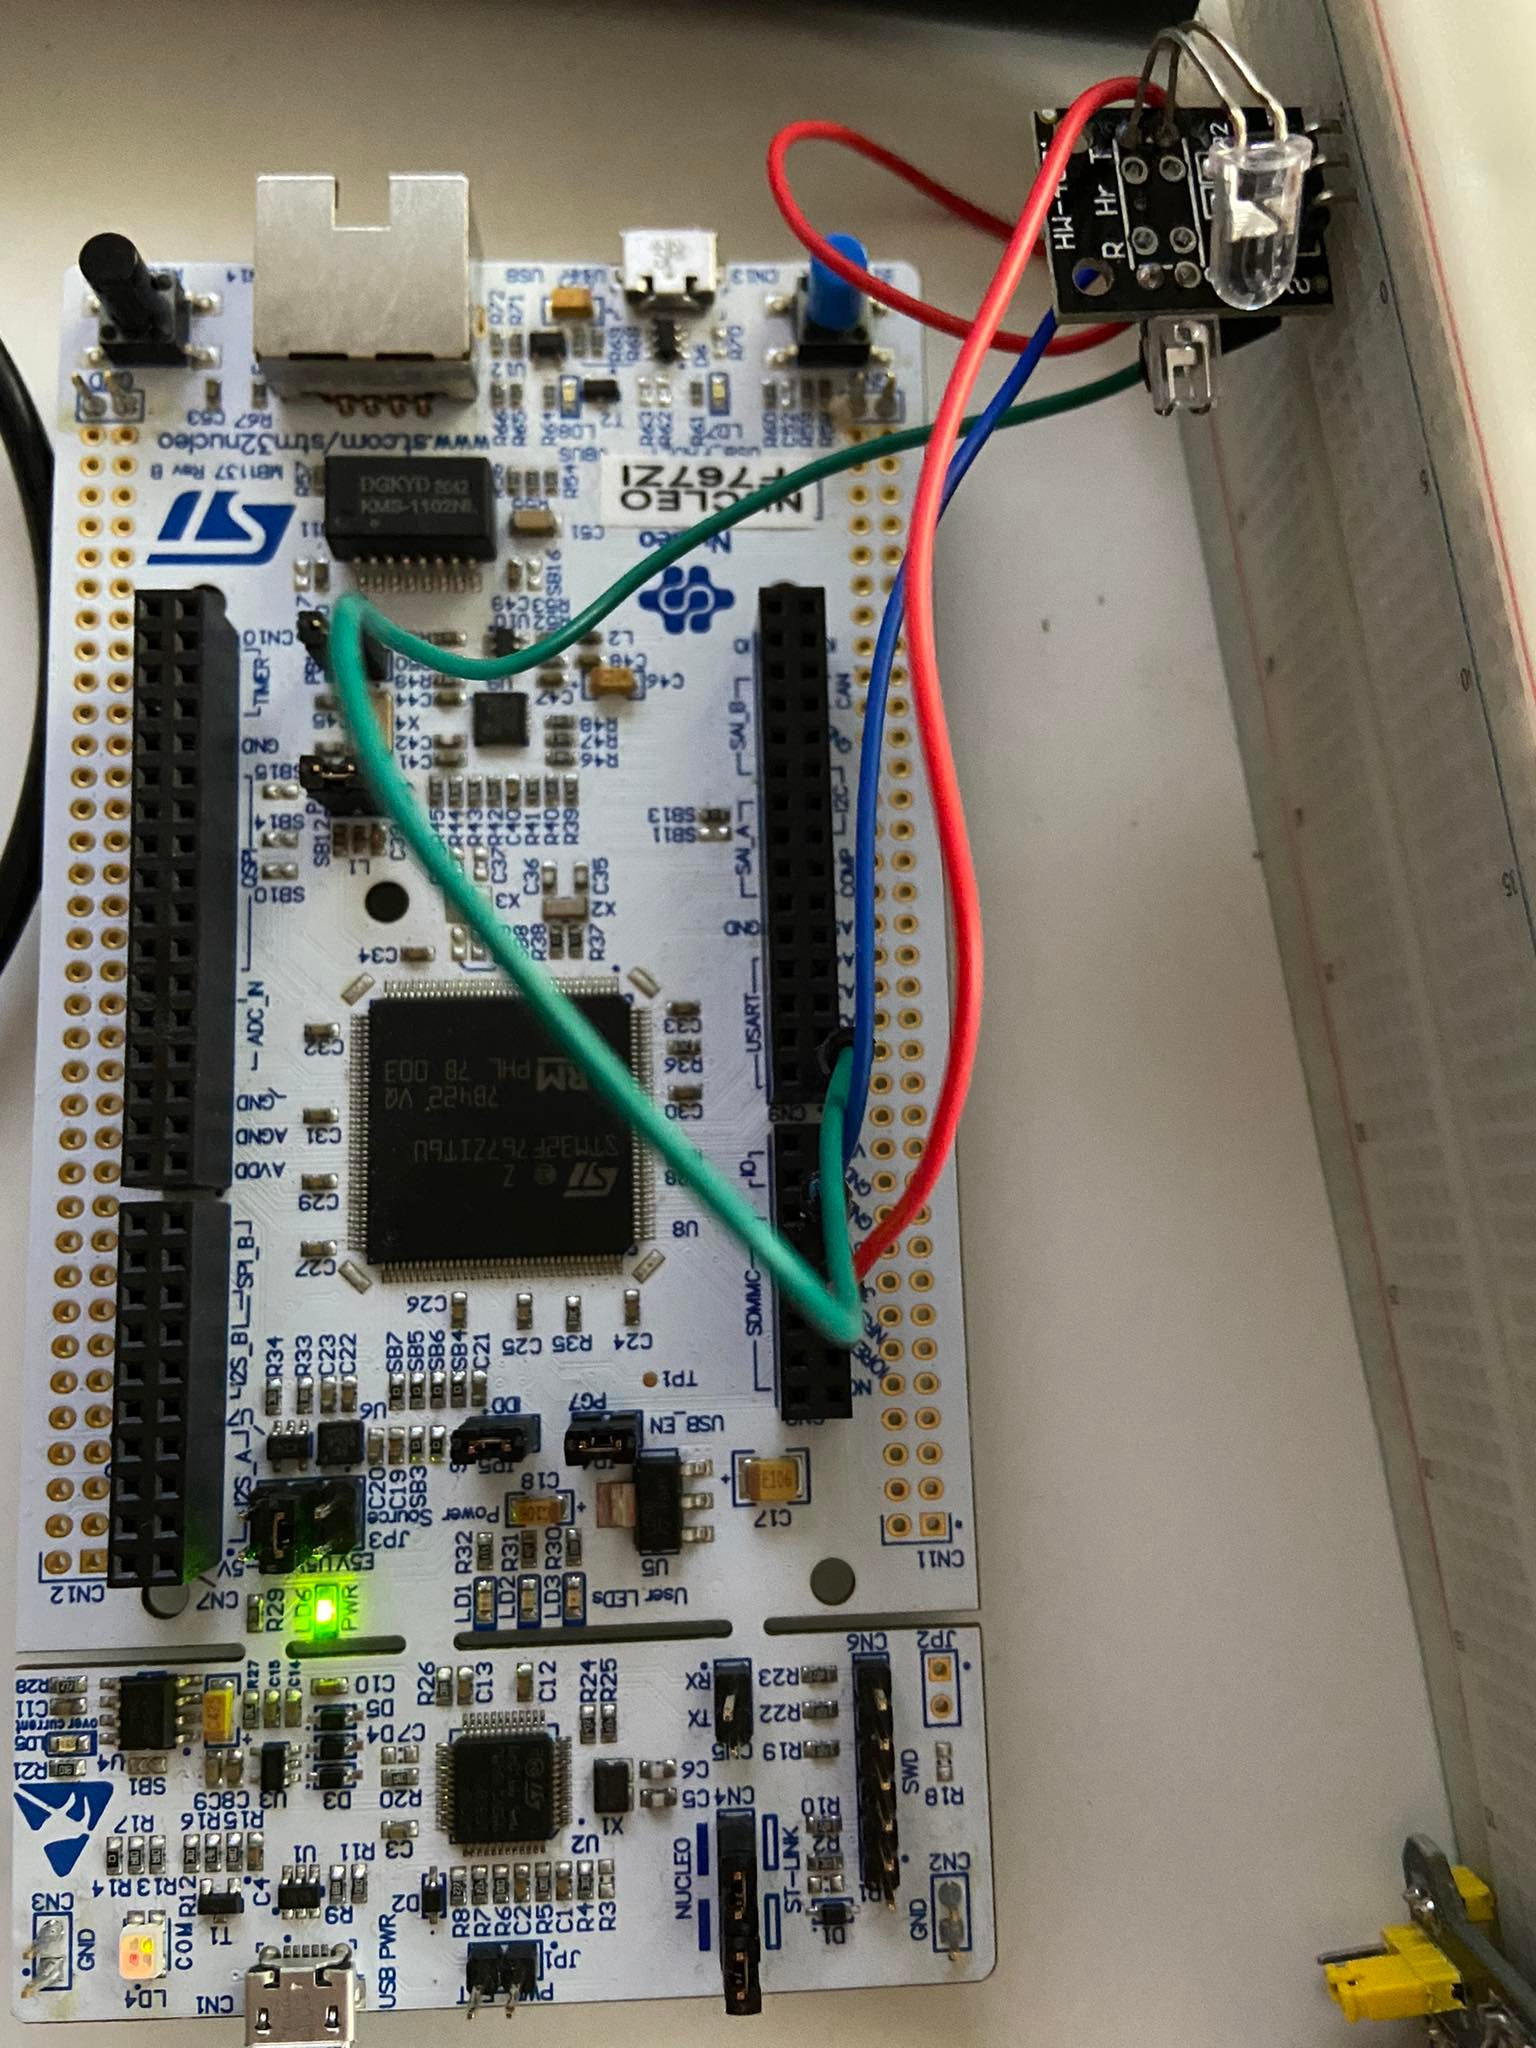
\includegraphics[width=0.9\linewidth]{fig/DS18B20/działanie_ukladu/zdj3.jpg}
\label{fig:_zdjecie_elementu}
\end{subfigure}%
%%%%%%%%%%%%%%%%%%%%%%%%%%%%%%%%%%%%%%%%%%%%%%%%%%%%%%%%%%%%%%%%%%%%%%%%%%%%%%%%%
\begin{subfigure}{.5\textwidth}
\centering
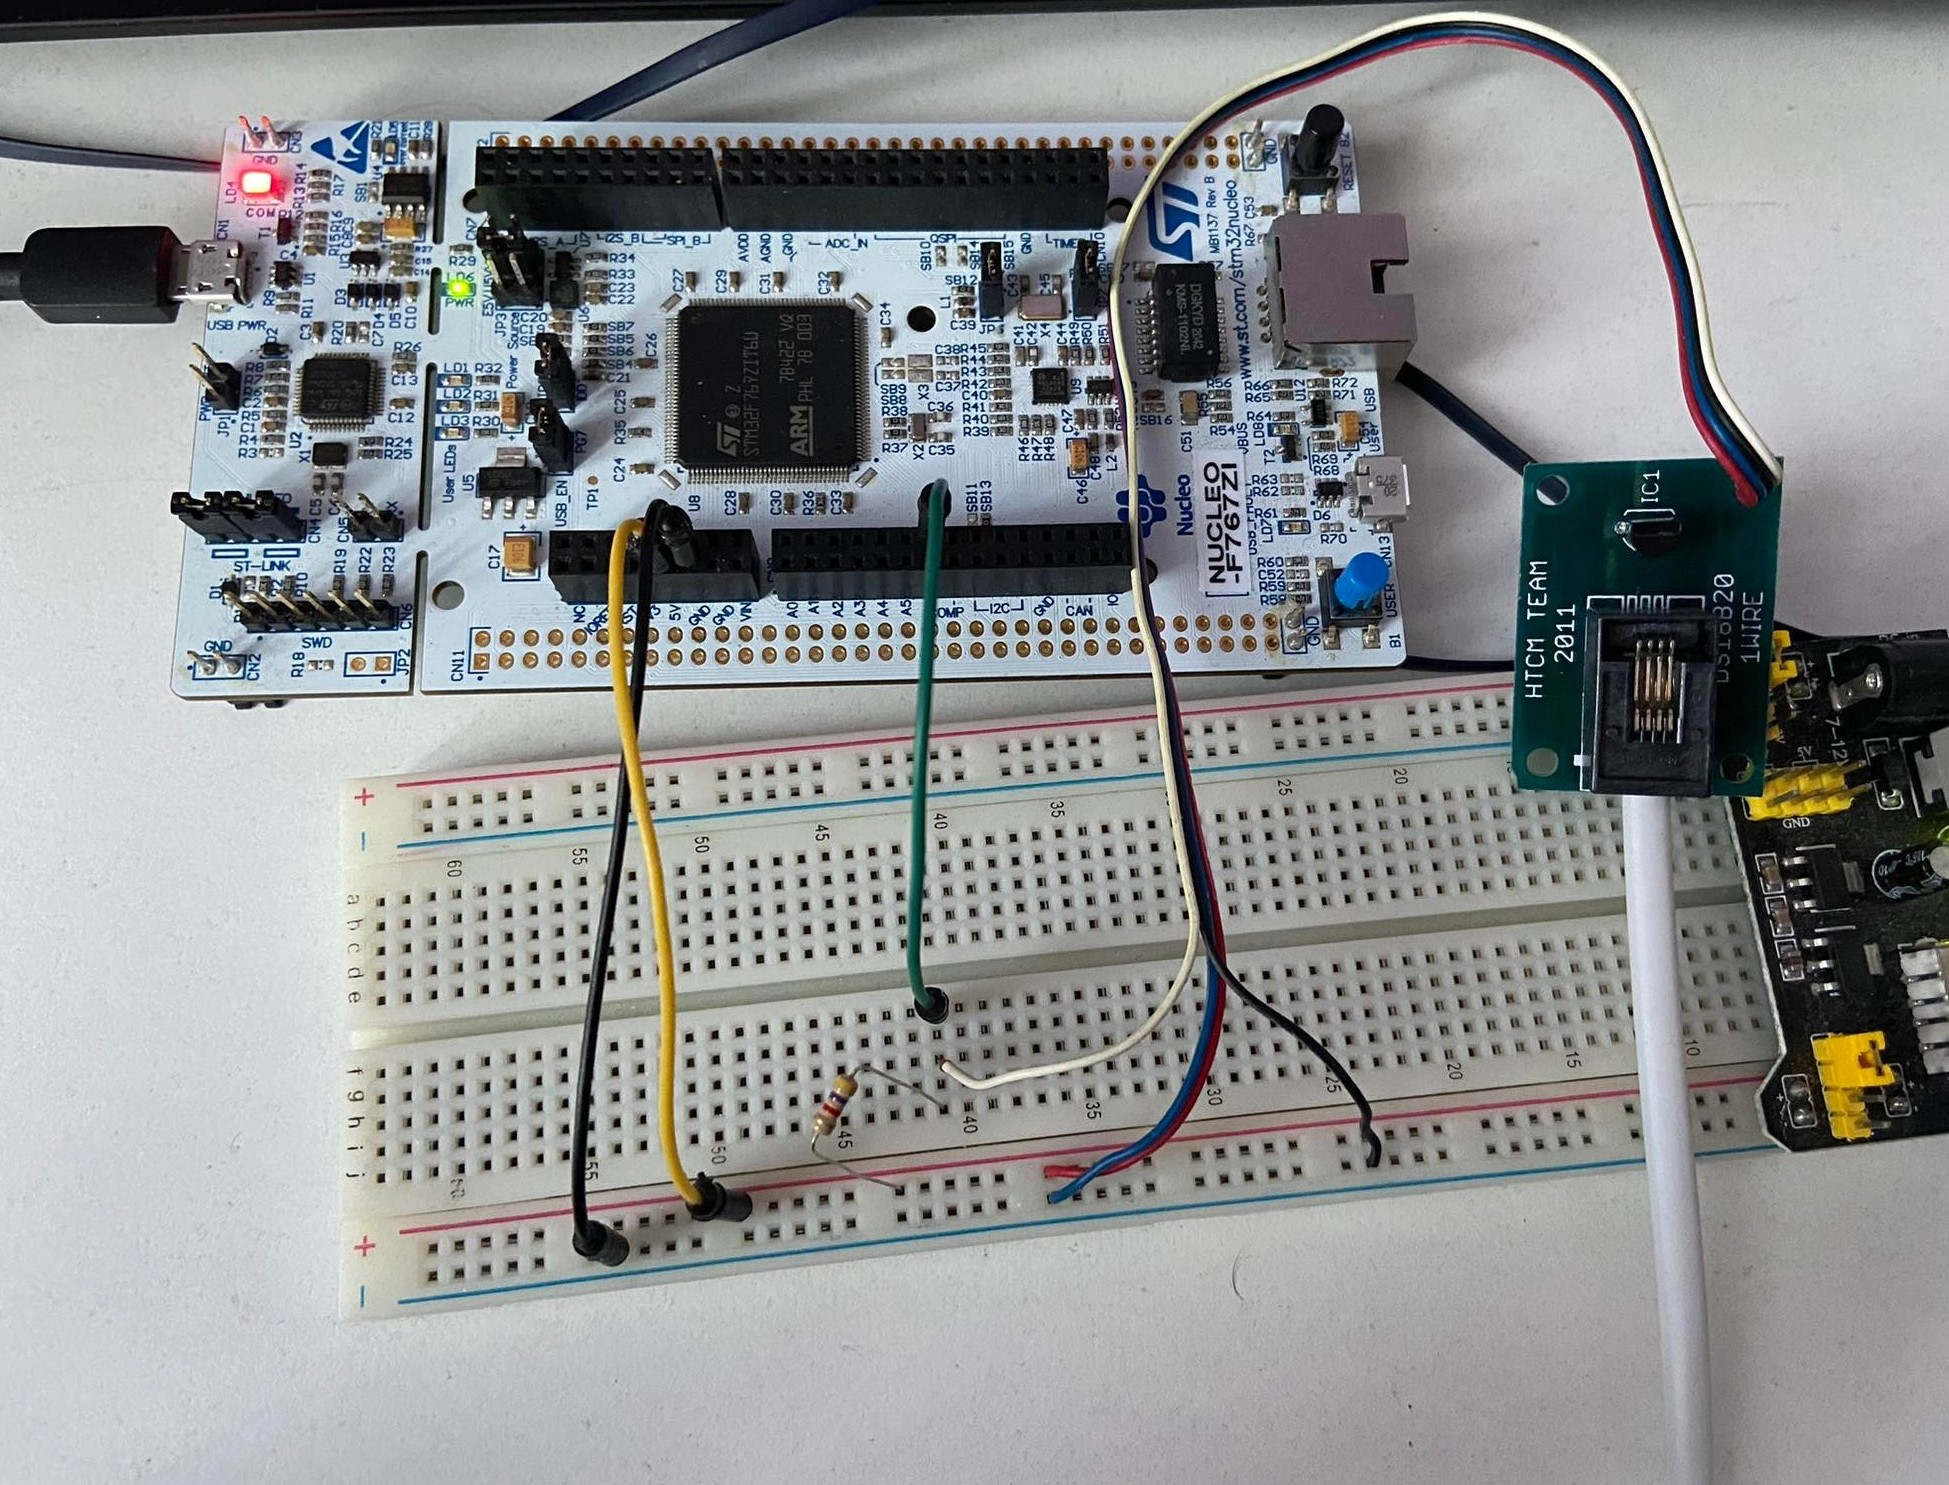
\includegraphics[width=0.9\linewidth]{fig/DS18B20/działanie_ukladu/zdj4.jpg}
\label{fig:_zasada_dzialania_elementu}
\end{subfigure}
\caption{Do spodu modułu zostały dolutowane przewody w celu podłączenia go do płytki stykowej.}
\end{figure}

Została zaprogramowana komunikacja typu OneWire do odczytu danych z czujnika.
\begin{figure}[h]
\centering
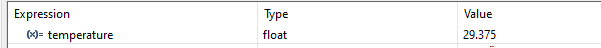
\includegraphics[width=\linewidth]{fig/DS18B20/działanie_ukladu/temperatura_pokoj.png}
\label{fig:_zdjecie_elementu}
\caption{Temperatura zmierzona w pomieszczeniu}
\end{figure}
\\
Następnie, czujnik został przyłożony do lampy w celu nagrzania, a logi pomiarów zostały wyświetlone przez UART w terminalu. 

%%%%%%%%%%%%%%%%%%%%%%%%%%%%%%%%%%%%%%%%%%%%%%%%%%%%%%%%%%%%%%%%%%%%%%%%%%%%%%%%%
\begin{figure}[h]
\begin{subfigure}{.5\textwidth}
\centering
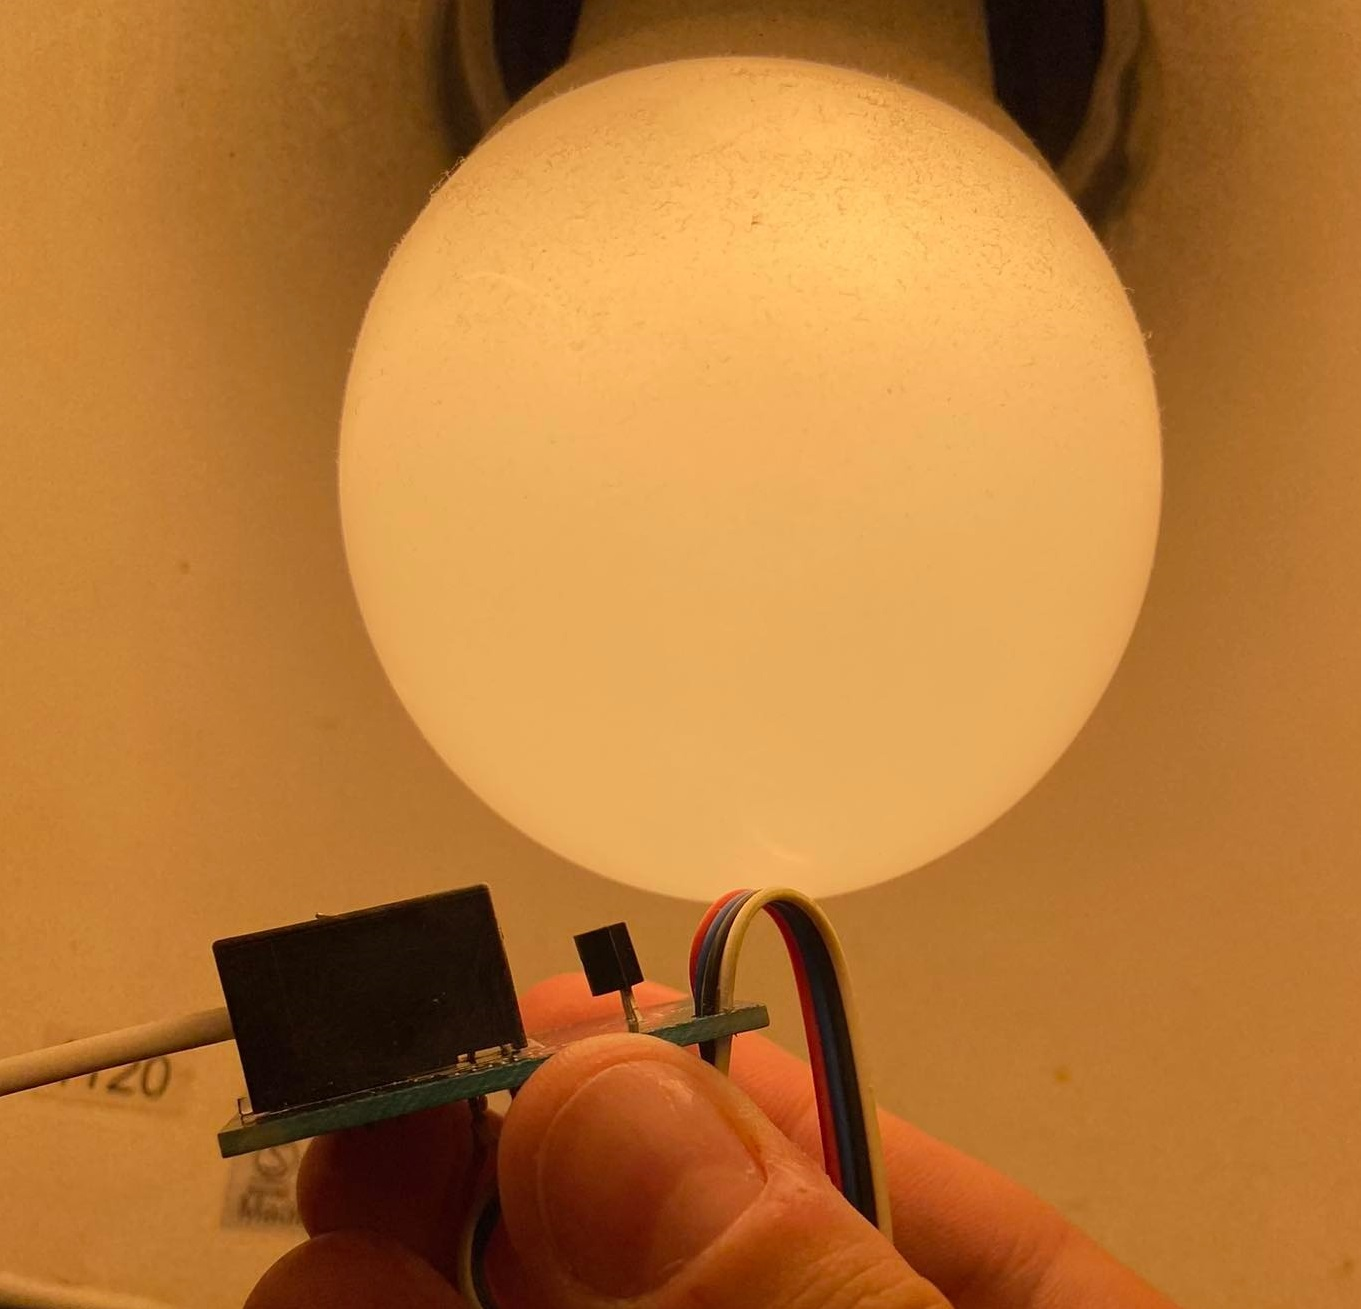
\includegraphics[width=0.8\linewidth]{fig/DS18B20/działanie_ukladu/zdj5.jpg}
\label{fig:_zdjecie_elementu}
\end{subfigure}%
%%%%%%%%%%%%%%%%%%%%%%%%%%%%%%%%%%%%%%%%%%%%%%%%%%%%%%%%%%%%%%%%%%%%%%%%%%%%%%%%%
\begin{subfigure}{.5\textwidth}
\centering
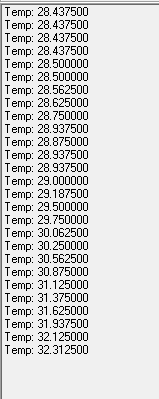
\includegraphics[width=0.3\linewidth]{fig/DS18B20/działanie_ukladu/logi.png}
\label{fig:_zasada_dzialania_elementu}
\end{subfigure}
\caption{Zgodnie z przewidywaniem, temperatura mierzona przez czujnik rośnie. }
\end{figure}


\newpage
\printbibliography[heading=bibintoc]

\end{document}